\subsection{Latency}
    In this test we measure the point-to-point latency between two MPI
    processes. By strategically selecting the allocation of these two,
    we can get a deeper insight on the latencies of our architecture.
    This approach is valuable also for understanding the impact
    of different topologies across each layer of the system.
    For each test we used the following parameters:
    \begin{itemize}
        \item iterations: 100
        \item warmup: 10
        \item message size: 1 byte to 1 Mb
    \end{itemize}
\subsubsection{Intra-Socket}
    In this test we bind the two processes to the same socket fixing
    the first to core 0 and varying the second from core 0 to core 11.
    Additionally we consider three different message sizes: 8 bytes,
    1 Kb, and 1 Mb. This way we obtain twelve measurements for each message
    size and we can analyze the impact of the message size on the latency.
    \begin{figure}[H]
        \centering
        \resizebox{0.45\textwidth}{!}{
        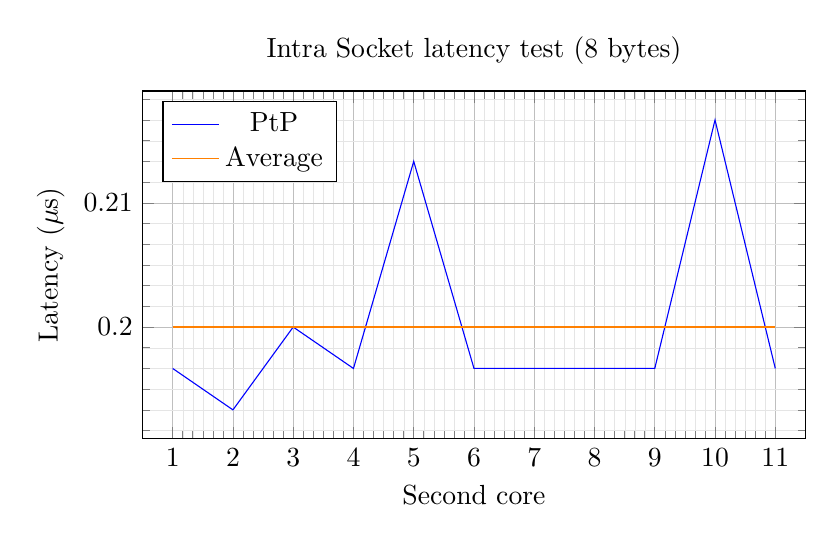
\begin{tikzpicture}
            \begin{axis}[
                title={Intra Socket latency test (8 bytes)},
                xlabel={Second core},
                ylabel={Latency ($\mu$s)},
                legend pos=north west,
                grid=both,
                grid style={line width=.1pt, draw=gray!20},
                major grid style={line width=.2pt,draw=gray!50},
                minor tick num=5,
                xtick={1, 2, 3, 4, 5, 6, 7, 8, 9, 10, 11},
                % xmode=log,
                % log basis x={2},
                % ymin=0,
                xmin=0.5,
                xmax=11.5,
                % xmax=100,
                % ytick={0, 50, 100, 150, 200, 250, 300, 350, 400},
                width=10cm,
                height=6cm,
                % cycle list name=color list,
            ]
            
            % x = [0,1,...,11]
            % y = [1.23599500e+04 1.96666667e-01 1.93333333e-01 2.00000000e-01 1.96666667e-01 2.13333333e-01 1.96666667e-01 1.96666667e-01 1.96666667e-01 1.96666667e-01 2.16666667e-01 1.96666667e-01]
            % avg = 0.19999999999999998
            % Blue line: Real
            \addplot[
                color=blue,
                mark=none,
                ]
                coordinates {
                (1, 0.196667)
                (2, 0.193333)
                (3, 0.200000)
                (4, 0.196667)
                (5, 0.213333)
                (6, 0.196667)
                (7, 0.196667)
                (8, 0.196667)
                (9, 0.196667)
                (10, 0.216667)
                (11, 0.196667)
                };
                \addlegendentry{PtP}
            
            % Orange line: Average
            \addplot[
                color=orange,
                mark=none,
                ]
                coordinates {
                (1, 0.19999999999999998)
                (11, 0.19999999999999998)
                };
                \addlegendentry{Average}
            
            \end{axis}
        \end{tikzpicture}
        }
    \end{figure}
    \begin{figure}[H]
        \centering
        \resizebox{0.45\textwidth}{!}{
        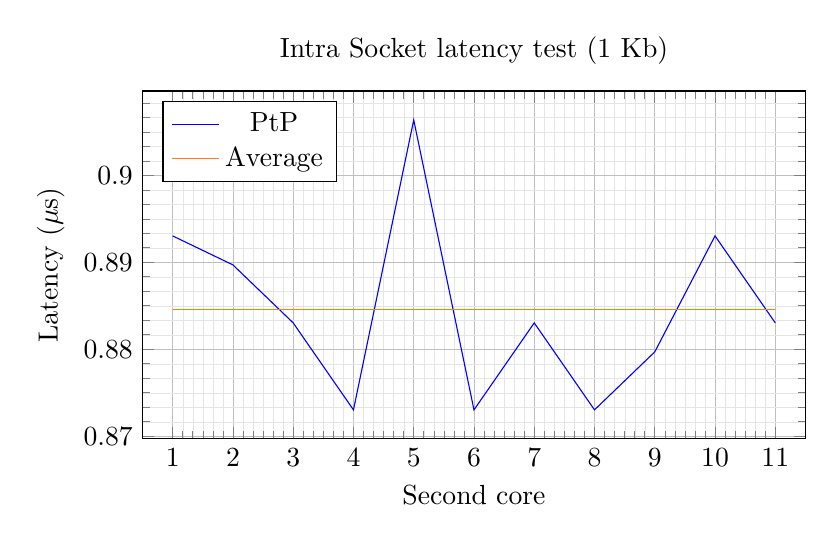
\begin{tikzpicture}
            \begin{axis}[
                title={Intra Socket latency test (1 Kb)},
                xlabel={Second core},
                ylabel={Latency ($\mu$s)},
                legend pos=north west,
                grid=both,
                grid style={line width=.1pt, draw=gray!20},
                major grid style={line width=.2pt,draw=gray!50},
                minor tick num=5,
                xtick={1, 2, 3, 4, 5, 6, 7, 8, 9, 10, 11},
                % xmode=log,
                % log basis x={2},
                % ymin=0,
                xmin=0.5,
                xmax=11.5,
                % xmax=100,
                % ytick={0, 50, 100, 150, 200, 250, 300, 350, 400},
                width=10cm,
                height=6cm,
                % cycle list name=color list,
            ]
            
            % x = [0,1,...,11]
            % y = [1.25343200e+04 8.93030303e-01 8.89696970e-01 8.83030303e-01 8.73030303e-01 9.06363636e-01 8.73030303e-01 8.83030303e-01 8.73030303e-01 8.79696970e-01 8.93030303e-01 8.83030303e-01 ]
            % avg = 0.8845454545454546
            % Blue line: Real
            \addplot[
                color=blue,
                mark=none,
                ]
                coordinates {
                (1, 0.893030)
                (2, 0.889697)
                (3, 0.883030)
                (4, 0.873030)
                (5, 0.906364)
                (6, 0.873030)
                (7, 0.883030)
                (8, 0.873030)
                (9, 0.879697)
                (10, 0.893030)
                (11, 0.883030)
                };
                \addlegendentry{PtP}
            
            % Orange line: Average
            \addplot[
                color=orange,
                mark=none,
                ]
                coordinates {
                (1, 0.8845454545454546)
                (11, 0.8845454545454546)
                };
                \addlegendentry{Average}
            
            \end{axis}
        \end{tikzpicture}
        }
    \end{figure}
    \begin{figure}[H]
        \centering
        \resizebox{0.45\textwidth}{!}{
        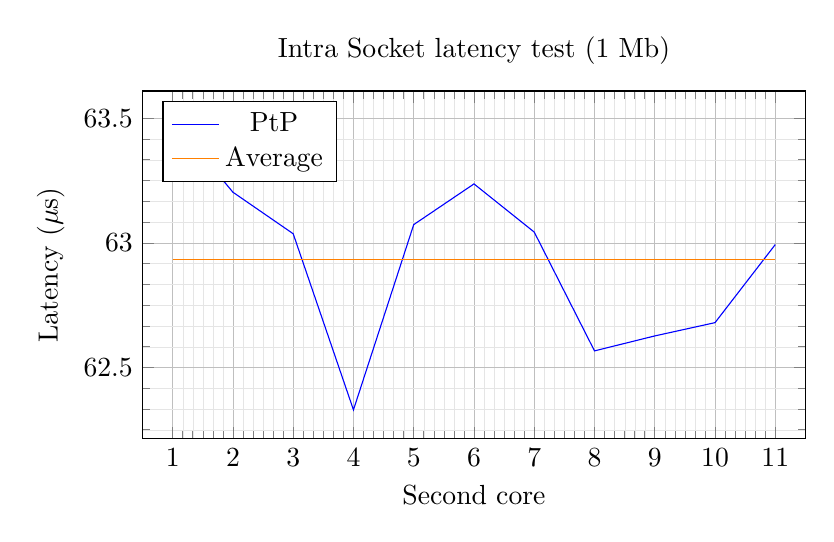
\begin{tikzpicture}
            \begin{axis}[
                title={Intra Socket latency test (1 Mb)},
                xlabel={Second core},
                ylabel={Latency ($\mu$s)},
                legend pos=north west,
                grid=both,
                grid style={line width=.1pt, draw=gray!20},
                major grid style={line width=.2pt,draw=gray!50},
                minor tick num=5,
                xtick={1, 2, 3, 4, 5, 6, 7, 8, 9, 10, 11},
                % xmode=log,
                % log basis x={2},
                % ymin=0,
                xmin=0.5,
                xmax=11.5,
                % xmax=100,
                % ytick={0, 50, 100, 150, 200, 250, 300, 350, 400},
                width=10cm,
                height=6cm,
                % cycle list name=color list,
            ]
            
            % x = [0,1,...,11]
            % y = [12189.89 63.4930303 63.2030303 63.03636364 62.32969697 63.0730303 63.23636364 63.0430303 62.56636364 62.62636364 62.67969697 62.9930303 ]
            % avg = 62.93454545454545
            % Blue line: Real
            \addplot[
                color=blue,
                mark=none,
                ]
                coordinates {
                (1, 63.4930303)
                (2, 63.2030303)
                (3, 63.03636364)
                (4, 62.32969697)
                (5, 63.0730303)
                (6, 63.23636364)
                (7, 63.0430303)
                (8, 62.56636364)
                (9, 62.62636364)
                (10, 62.67969697)
                (11, 62.9930303)
                };
                \addlegendentry{PtP}
            
            % Orange line: Average
            \addplot[
                color=orange,
                mark=none,
                ]
                coordinates {
                (1, 62.93454545454545)
                (11, 62.93454545454545)
                };
                \addlegendentry{Average}
            
            \end{axis}
        \end{tikzpicture}
        }
    \end{figure}
    The communication is the slowest when the second process is bound
    to the same core as the first process. We do not represet this
    value in the plot for readability reasons. Hereafter we report
    some further statistics:
    % Table
    \begin{table}[H]
        \centering
        \begin{tabular}{|c|c|c|c|}
            \hline
            \textbf{Message size} & \textbf{Average ($\mu$s)} & \textbf{Std ($\mu$s)} & \textbf{Std/Average} \\
            \hline
            8 bytes & 0.19 & 0.007 & 0.0362 \\
            1 Kb & 0.88 & 0.009 & 0.0111 \\
            1 Mb & 62.93 & 0.33 & 0.005 \\
            \hline
        \end{tabular}
    \end{table}
    As we can see, the absolute variability of the latency increases
    with the message size. However, if we consider the relative
    variability, we can see that the latency is more stable for larger
    messages.
    Finally, we analyze all the tested message sizes averaging the
    latencies among each core combination.
    \begin{figure}[H]
        \centering
        \resizebox{0.45\textwidth}{!}{
        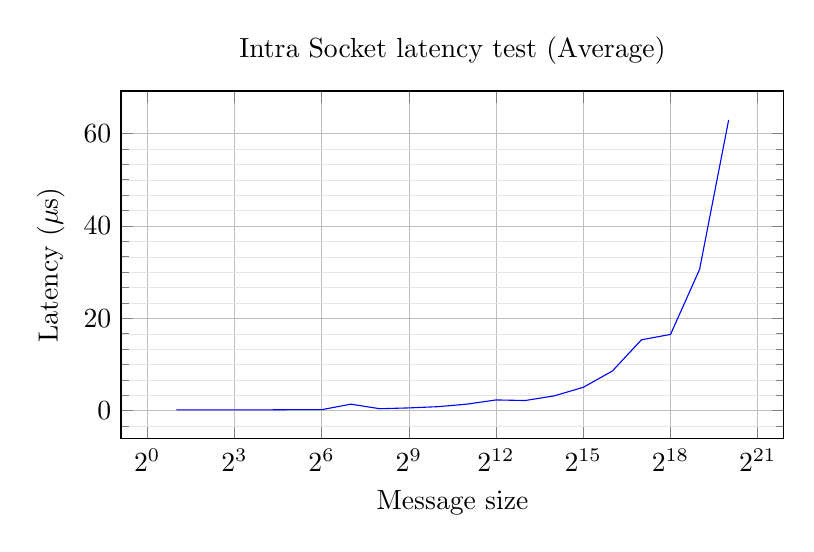
\begin{tikzpicture}
            \begin{axis}[
                title={Intra Socket latency test (Average)},
                xlabel={Message size},
                ylabel={Latency ($\mu$s)},
                legend pos=north west,
                grid=both,
                grid style={line width=.1pt, draw=gray!20},
                major grid style={line width=.2pt,draw=gray!50},
                minor tick num=5,
                % xtick={1, 2, 3, 4, 5, 6, 7, 8, 9, 10, 11},
                xmode=log,
                log basis x={2},
                % ymin=0,
                % xmin=0.5,
                % xmax=11.5,
                % xmax=100,
                % ytick={0, 50, 100, 150, 200, 250, 300, 350, 400},
                width=10cm,
                height=6cm,
                % cycle list name=color list,
            ]
            
            % x = [[      2,       4,       8,      16,      32,      64,     128,     256,           512,    1024,    2048,    4096,    8192,   16384,   32768,   65536, 131072,  262144,  524288, 1048576]
            % y = [ 0.19181818  0.19636364  0.2         0.19090909  0.24090909  0.23272727  1.42545455  0.44272727  0.61818182  0.88454545  1.43636364  2.34272727  2.21636364  3.22181818  5.07454545  8.59727273 15.35272727 16.52272727 30.58909091 62.93454545]
            % Blue line: Real
            \addplot[
                color=blue,
                mark=none,
                ]
                coordinates {
                (2, 0.19181818)
                (4, 0.19636364)
                (8, 0.2)
                (16, 0.19090909)
                (32, 0.24090909)
                (64, 0.23272727)
                (128, 1.42545455)
                (256, 0.44272727)
                (512, 0.61818182)
                (1024, 0.88454545)
                (2048, 1.43636364)
                (4096, 2.34272727)
                (8192, 2.21636364)
                (16384, 3.22181818)
                (32768, 5.07454545)
                (65536, 8.59727273)
                (131072, 15.35272727)
                (262144, 16.52272727)
                (524288, 30.58909091)
                (1048576, 62.93454545)
                };
            
            \end{axis}
        \end{tikzpicture}
        }
    \end{figure}
    Even with the significant increase in the latency for larger messages,
    its growth is not exponential. This is clearer
    when we consider the linear scale of the plot.
    \begin{figure}[H]
        \centering
        \resizebox{0.45\textwidth}{!}{
        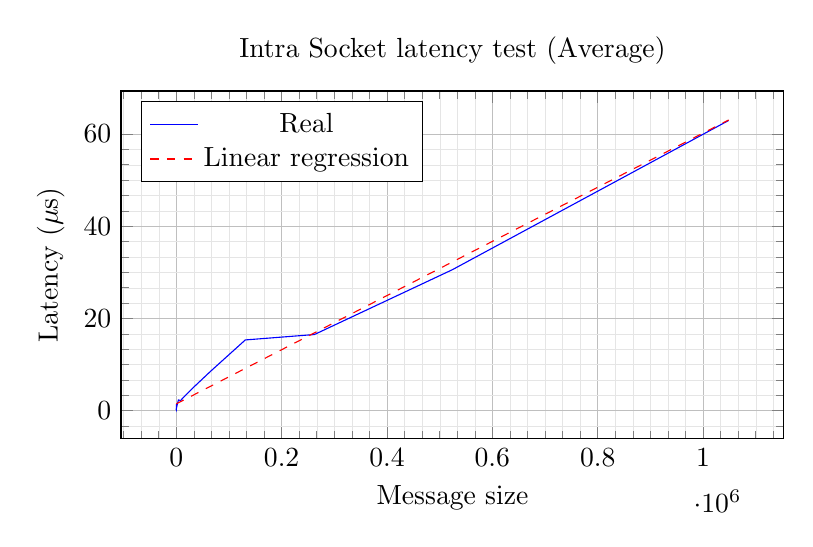
\begin{tikzpicture}
            \begin{axis}[
                title={Intra Socket latency test (Average)},
                xlabel={Message size},
                ylabel={Latency ($\mu$s)},
                legend pos=north west,
                grid=both,
                grid style={line width=.1pt, draw=gray!20},
                major grid style={line width=.2pt,draw=gray!50},
                minor tick num=5,
                % xtick={1, 2, 3, 4, 5, 6, 7, 8, 9, 10, 11},
                % xmode=log,
                % log basis x={2},
                % ymin=0,
                % xmin=0.5,
                % xmax=11.5,
                % xmax=100,
                % ytick={0, 50, 100, 150, 200, 250, 300, 350, 400},
                width=10cm,
                height=6cm,
                % cycle list name=color list,
            ]
            
            % x = [[      2,       4,       8,      16,      32,      64,     128,     256,           512,    1024,    2048,    4096,    8192,   16384,   32768,   65536, 131072,  262144,  524288, 1048576]
            % y = [ 0.19181818  0.19636364  0.2         0.19090909  0.24090909  0.23272727  1.42545455  0.44272727  0.61818182  0.88454545  1.43636364  2.34272727  2.21636364  3.22181818  5.07454545  8.59727273 15.35272727 16.52272727 30.58909091 62.93454545]
            % linreg = [ 1.49000803  1.49012544  1.49036026  1.49082991  1.49176919  1.49364777  1.49740491  1.5049192   1.51994778  1.55000494  1.61011926  1.73034789  1.97080516  2.45171971  3.4135488   5.33720697  9.18452332 16.87915602 32.26842142 63.04695221]
            % Blue line: Real
            \addplot[
                color=blue,
                mark=none,
                ]
                coordinates {
                (2, 0.19181818)
                (4, 0.19636364)
                (8, 0.2)
                (16, 0.19090909)
                (32, 0.24090909)
                (64, 0.23272727)
                (128, 1.42545455)
                (256, 0.44272727)
                (512, 0.61818182)
                (1024, 0.88454545)
                (2048, 1.43636364)
                (4096, 2.34272727)
                (8192, 2.21636364)
                (16384, 3.22181818)
                (32768, 5.07454545)
                (65536, 8.59727273)
                (131072, 15.35272727)
                (262144, 16.52272727)
                (524288, 30.58909091)
                (1048576, 62.93454545)
                };
            \addlegendentry{Real}

            % Red line: Linear regression
            % dashe
            \addplot[
                color=red,
                mark=none,
                dashed
                ]
                coordinates {
                (2, 1.49000803)
                (4, 1.49012544)
                (8, 1.49036026)
                (16, 1.49082991)
                (32, 1.49176919)
                (64, 1.49364777)
                (128, 1.49740491)
                (256, 1.5049192)
                (512, 1.51994778)
                (1024, 1.55000494)
                (2048, 1.61011926)
                (4096, 1.73034789)
                (8192, 1.97080516)
                (16384, 2.45171971)
                (32768, 3.4135488)
                (65536, 5.33720697)
                (131072, 9.18452332)
                (262144, 16.87915602)
                (524288, 32.26842142)
                (1048576, 63.04695221)
                };
            \addlegendentry{Linear regression}
            
            \end{axis}
        \end{tikzpicture}
        }
    \end{figure}
    The data clearly exhibits a linear behaviour, with a slope of
    approximately $58.7 \mu$s/MB, starting from the intercept with
    value $1.49 \mu$s. This means that the latency grows linearly
    This simple yet effective model enable us to estimate the latency
    for larger messages, assuming the linearity of the system will
    still hold. The only deviation is for the smallest message size,
    where the latency is more than linear. This could be due to the
    overhead of the communication system, which is more significant
    for smaller messages.


\subsubsection{Intra-Node}
    In this test we bind the two processes to different sockets. We fix
    the first process to socket 0 core 0 and the second process to socket
    1 core 0. We vary the second process from core 0 to core 3, 6, and 10.
    We again expect the latency to be stable across the different cores and
    this is the reason we tested only four of them. Since we have less test
    points we directly report a table.
    % Table
    \begin{table}[H]
        \centering
        \begin{tabular}{|c|c|c|c|}
            \hline
            \textbf{Message size} & \textbf{Average ($\mu$s)} & \textbf{Std ($\mu$s)} & \textbf{Std/Average} \\
            \hline
            8 bytes & 0.405 & 0.005 & 0.0123 \\
            1 Kb & 1.9175 & 0.0217 & 0.0113 \\
            1 Mb & 63.6575 & 0.8918 & 0.0140 \\
            \hline
        \end{tabular}
    \end{table}
    This time we observe a different behaviour in the variability-to-average
    ratio. Instead of decreasing as in the previous test, it stays almost
    constant around an average of $0.0125$. Having seen the previous result,
    we ask ourselves if again the latency grows linearly with the message size.
    \begin{figure}[H]
        \centering
        \resizebox{0.45\textwidth}{!}{
        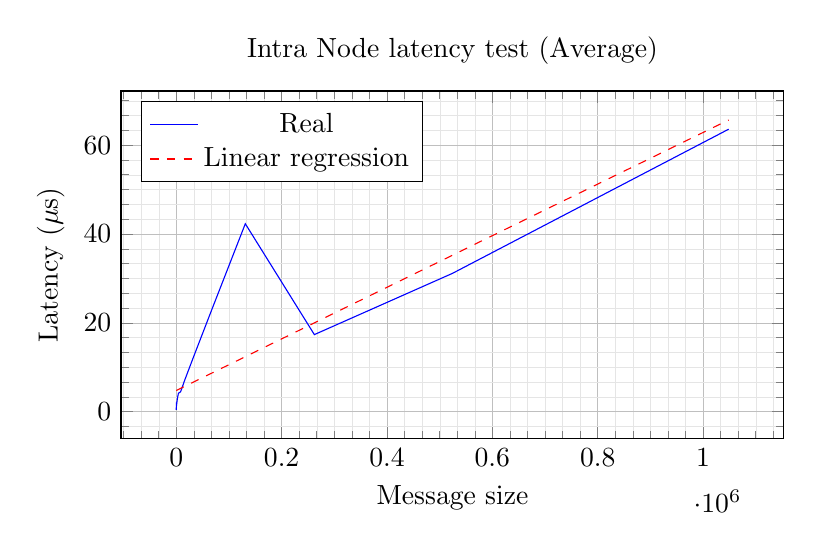
\begin{tikzpicture}
            \begin{axis}[
                title={Intra Node latency test (Average)},
                xlabel={Message size},
                ylabel={Latency ($\mu$s)},
                legend pos=north west,
                grid=both,
                grid style={line width=.1pt, draw=gray!20},
                major grid style={line width=.2pt,draw=gray!50},
                minor tick num=5,
                % xtick={1, 2, 3, 4, 5, 6, 7, 8, 9, 10, 11},
                % xmode=log,
                % log basis x={2},
                % ymin=0,
                % xmin=0.5,
                % xmax=11.5,
                % xmax=100,
                % ytick={0, 50, 100, 150, 200, 250, 300, 350, 400},
                width=10cm,
                height=6cm,
                % cycle list name=color list,
            ]
            
            % x = [[      2,       4,       8,      16,      32,      64,     128,     256,           512,    1024,    2048,    4096,    8192,   16384,   32768,   65536, 131072,  262144,  524288, 1048576]
            % y = [ 0.41        0.4         0.40666667  0.41333333  0.57        0.58  2.08333333  1.14666667  1.42666667  1.92666667  2.85333333  4.14666667  4.46        7.20333333 12.32       22.38666667 42.30333333 17.35 31.13333333 63.58666667]
            % linreg = [ 4.76505022  4.76516638  4.76539871  4.76586337  4.76679269  4.76865134  4.77236863  4.7798032   4.79467236  4.82441066  4.88388727  5.0028405  5.24074695  5.71655985  6.66818564  8.57143723 12.37794041 19.99094678 35.21695951 65.66898497]
            % Blue line: Real
            \addplot[
                color=blue,
                mark=none,
                ]
                coordinates {
                (2, 0.41)
                (4, 0.4)
                (8, 0.40666667)
                (16, 0.41333333)
                (32, 0.57)
                (64, 0.58)
                (128, 2.08333333)
                (256, 1.14666667)
                (512, 1.42666667)
                (1024, 1.92666667)
                (2048, 2.85333333)
                (4096, 4.14666667)
                (8192, 4.46)
                (16384, 7.20333333)
                (32768, 12.32)
                (65536, 22.38666667)
                (131072, 42.30333333)
                (262144, 17.35)
                (524288, 31.13333333)
                (1048576, 63.58666667)
                };
            \addlegendentry{Real}

            % Red line: Linear regression
            % dashe
            \addplot[
                color=red,
                mark=none,
                dashed
                ]
                coordinates {
                (2, 4.76505022)
                (4, 4.76516638)
                (8, 4.76539871)
                (16, 4.76586337)
                (32, 4.76679269)
                (64, 4.76865134)
                (128, 4.77236863)
                (256, 4.7798032)
                (512, 4.79467236)
                (1024, 4.82441066)
                (2048, 4.88388727)
                (4096, 5.0028405)
                (8192, 5.24074695)
                (16384, 5.71655985)
                (32768, 6.66818564)
                (65536, 8.57143723)
                (131072, 12.37794041)
                (262144, 19.99094678)
                (524288, 35.21695951)
                (1048576, 65.66898497)
                };
            \addlegendentry{Linear regression}
            
            \end{axis}
        \end{tikzpicture}
        }
    \end{figure}
    This time, even if starting from a higher intercept of value
    $4.76 \mu$s, the slope is approximately the same as the previous
    test, around $58.7 \mu$s/MB. This means that not only the latency
    grows linearly with the message size, but also the rate of growth
    is the same as in the previous test. This is a very interesting
    result, since it means that the latency is not only stable across
    different cores, but also across different sockets. However, the
    non-linear behaviour for the smallest message size is now more evident.

\subsubsection{Intra-Cluster}
    Finally we test the latency between two processes on different nodes.
    We test the following combinations:
    \begin{itemize}
        \item N0 S0 C0 $\leftrightarrow$ N1 S0 C0
        \item N0 S0 C0 $\leftrightarrow$ N1 S1 C0
        \item N0 S1 C0 $\leftrightarrow$ N1 S0 C0
        \item N0 S1 C0 $\leftrightarrow$ N1 S1 C0
    \end{itemize}
    Again we report the results in a table.
    \begin{table}[H]
        \centering
        \begin{tabular}{|c|c|c|c|}
            \hline
            \textbf{Message size} & \textbf{Average ($\mu$s)} & \textbf{Std ($\mu$s)} & \textbf{Std/Average} \\
            \hline
            8 bytes & 1.1250 & 0.0622 & 0.0553 \\
            1 Kb & 1.9550 & 0.1484 & 0.0759 \\
            1 Mb & 94.2250 & 0.3829 & 0.0041 \\
            \hline
        \end{tabular}
    \end{table}
    This time we observe again a different behaviour in the variability-to-average
    ratio. It increases when considering low values of the message size and
    then drops for larger values becoming more and more stable.\\
    Once more we check for the linearity of the latency with the message size.
    \begin{figure}[H]
        \centering
        \resizebox{0.45\textwidth}{!}{
        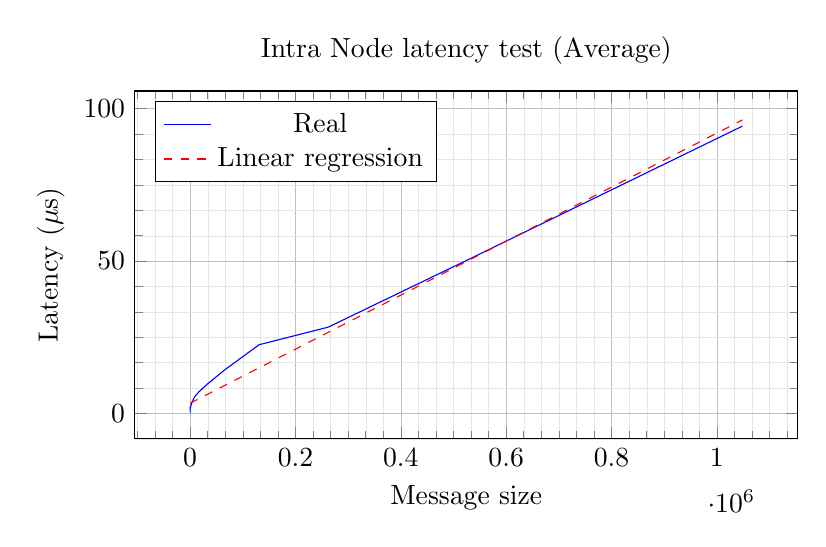
\begin{tikzpicture}
            \begin{axis}[
                title={Intra Node latency test (Average)},
                xlabel={Message size},
                ylabel={Latency ($\mu$s)},
                legend pos=north west,
                grid=both,
                grid style={line width=.1pt, draw=gray!20},
                major grid style={line width=.2pt,draw=gray!50},
                minor tick num=5,
                % xtick={1, 2, 3, 4, 5, 6, 7, 8, 9, 10, 11},
                % xmode=log,
                % log basis x={2},
                % ymin=0,
                % xmin=0.5,
                % xmax=11.5,
                % xmax=100,
                % ytick={0, 50, 100, 150, 200, 250, 300, 350, 400},
                width=10cm,
                height=6cm,
                % cycle list name=color list,
            ]
            
            % x = [[      2,       4,       8,      16,      32,      64,     128,     256,           512,    1024,    2048,    4096,    8192,   16384,   32768,   65536, 131072,  262144,  524288, 1048576]
            % y = [ 1.16666667  1.13333333  1.14333333  1.13666667  1.19333333  1.41  1.5         1.74        1.83        2.02333333  2.80666667  3.79666667  5.32666667  7.01333333  9.60333333 14.25       22.52666667 28.29333333 50.15666667 94.30333333]
            % linreg = [ 3.31773287  3.31791025  3.31826502  3.31897457  3.32039365  3.32323182  3.32890816  3.34026085  3.36296622  3.40837696  3.49919845  3.68084142  4.04412736  4.77069924  6.223843    9.13013051 14.94270555 26.56785562 49.81815576 96.31875605]
            % Blue line: Real
            \addplot[
                color=blue,
                mark=none,
                ]
                coordinates {
                (2, 1.16666667)
                (4, 1.13333333)
                (8, 1.14333333)
                (16, 1.13666667)
                (32, 1.19333333)
                (64, 1.41)
                (128, 1.5)
                (256, 1.74)
                (512, 1.83)
                (1024, 2.02333333)
                (2048, 2.80666667)
                (4096, 3.79666667)
                (8192, 5.32666667)
                (16384, 7.01333333)
                (32768, 9.60333333)
                (65536, 14.25)
                (131072, 22.52666667)
                (262144, 28.29333333)
                (524288, 50.15666667)
                (1048576, 94.30333333)
                };
            \addlegendentry{Real}

            % Red line: Linear regression
            % dashe
            \addplot[
                color=red,
                mark=none,
                dashed
                ]
                coordinates {
                (2, 3.31773287)
                (4, 3.31791025)
                (8, 3.31826502)
                (16, 3.31897457)
                (32, 3.32039365)
                (64, 3.32323182)
                (128, 3.32890816)
                (256, 3.34026085)
                (512, 3.36296622)
                (1024, 3.40837696)
                (2048, 3.49919845)
                (4096, 3.68084142)
                (8192, 4.04412736)
                (16384, 4.77069924)
                (32768, 6.223843)
                (65536, 9.13013051)
                (131072, 14.94270555)
                (262144, 26.56785562)
                (524288, 49.81815576)
                (1048576, 96.31875605)
                };
            \addlegendentry{Linear regression}
            
            \end{axis}
        \end{tikzpicture}
        }
    \end{figure}
    Suprisingly, the intercept of this last model is lower than the previous
    one. Obviously computing the latency for an empty message is not realistic,
    therefore this value should be taken with caution. However, the slope is
    $88.69 \mu$s/MB, which is higher than the previous tests. The initial 
    deviation is suppressed by the higher slope making it less noticeable.


